\section{Backgrounds}
\label{sect:bkgLepTau}
In different channels, the contribution of the events with a fake \Tau, namely QCD and $W$jets is estimated using the data. 
For the prompt \Tau's, from top, $\cPZ$jets, di-boson and higgs we trust 
the MC, but the important contributions are validated in a signal like region. 
In this section we will discuss the different background estimation techniques used.
%In continue, estimation of different backgrounds are explained.

\subsection{\texorpdfstring{QCD background estimation in $\tauTau$ channel}{QCD background estimation in tau-tau channel}}
%Due to the large cross section of the QCD multijet events and lack of the statistics, there is a large statistical uncertainty on the 
%yield of the QCD events from MC. On the other hand, 
The QCD multijet events contribute to the signal selection of the \tauTau channel, when two jets are 
fakely identified as \Tau's. The fake rate can be different between data and MC, so a data driven method is developed to estimate the 
contribution of the QCD multijet events. 
Since the search variable (\mttwo in \binone and \SumMT in \bintwo) and the 
isolation of the \Tau's are uncorrelated in the QCD events, the ratio of the events selected by the signal cuts over the events 
with loosely isolated \Tau's should be independent from the search variable, so one can find the ratio in the low \mttwo or \SumMT and 
multiply it to the number of events in the control region which is defined same as the signal region except the \Tau's are loosely isolated. 
This would give an estimate of the QCD events in the signal region. In the signal region, loosely isolated  \Tau's 
%($I_{\Tau} <$ 2 \GeV ) 
are excluded, but in the control region, only the pairs with at least one loosely isolated \Tau are selected. 
These pairs are requested to be same-sign to suppress the signal contamination. To further increase the statistics 
in different regions, the cut on the minimum angle in the transverse plane between the \MET and the jets is removed. The final estimation
is corrected by the efficiency of this cut which is read from data and will be described in continue.
Figure \ref{fig:ABCDQCD} shows different regions discussed here, schematically.
\begin{figure}[!Hhtb]
\centering
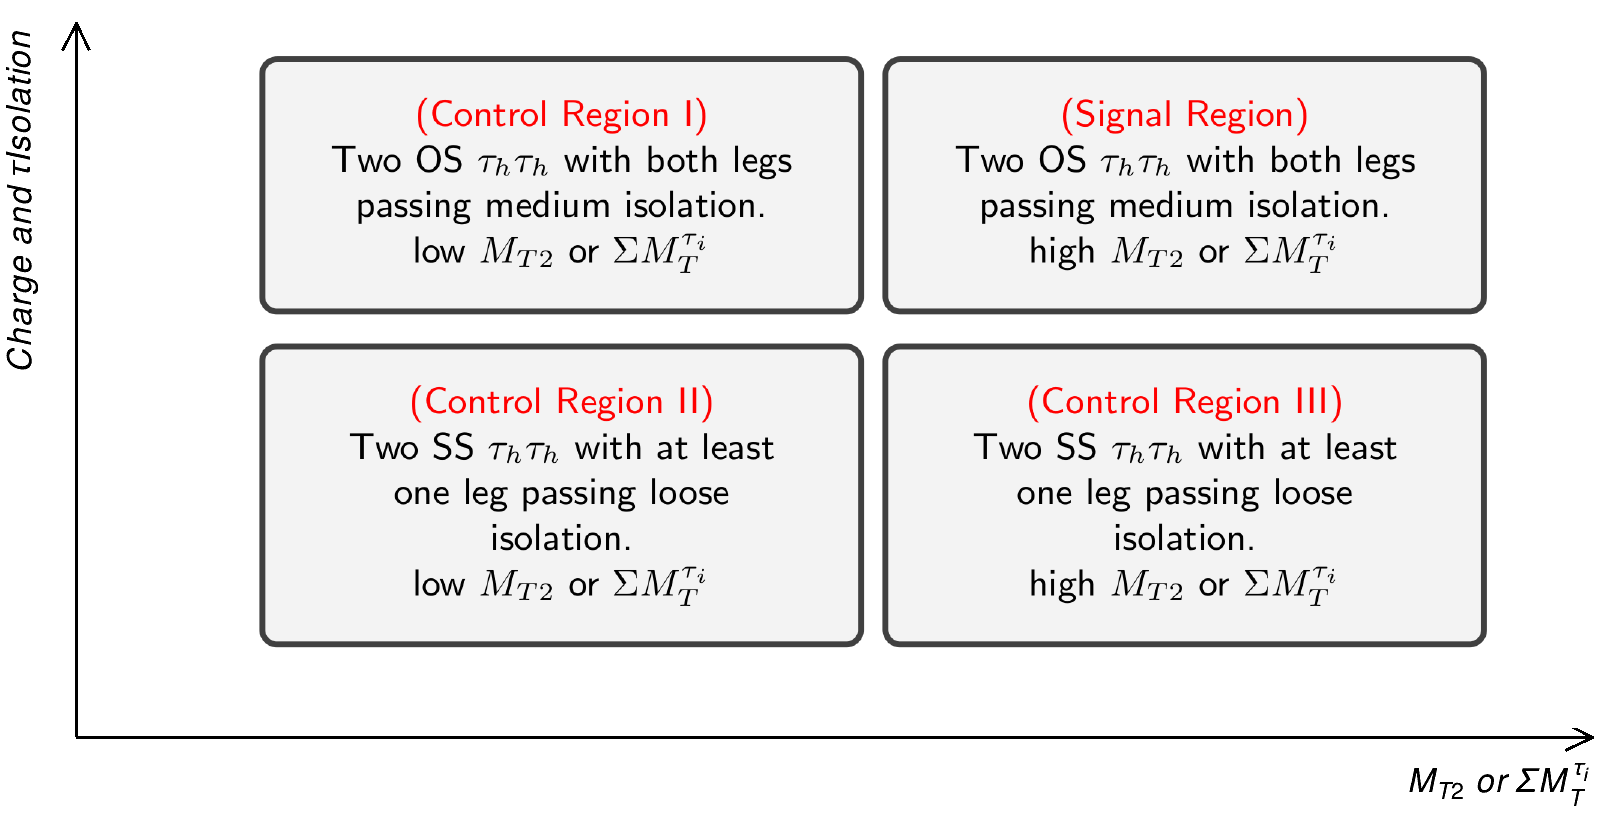
\includegraphics[angle=0,scale=0.30]{Bkg/ABCD.png}
\caption{Schematic description of the regions used to estimate the QCD backgrounds.}
\label{fig:ABCDQCD}
\end{figure}

Non-QCD events from MC are subtracted from data to find a QCD sample.
In the low \mttwo or \SumMT of the QCD sample, the ratio of the signal like events over the same-sign loose pairs 
is found and verified to be flat as a function of the search variable. 
%A horizontal line is fitted to
This ratio is multiplied to the same-sign loose pairs in high \mttwo or \SumMT and corrected by the efficiency of the 
cut on the minimum angle between the \MET and the jets, to find the QCD contamination in the signal region. 
The efficiency of the cut on the minimum angle between the \MET and the jets, is found with the same events as a function of the search variables.
The value of the efficiency in the last bin in vicinity of the signal region is used to correct the estimation.
To estimate the systematic uncertainty of the estimated value and take into account the potential correlation between the two values, 
the method to extract the
ratio and the efficiency are varied from approximating by a flat line to fitting by a straight line with a floating slope 
or using the value of the  last bin before the signal region. 
%This is  also a measure  of the correlation between the two variables which are assumed to be uncorrelated. 
Table \ref{4QCDbg} 
\begin{table}[!Hhtb]
\begin{center}
\begin{tabular}{|l|c|}
\hline\hline
 Region      &  Estimation\\
\hline\hline
\binone      & 0.15 $\pm$ 0.22 $\pm$ 0.13 \\
\hline
\bintwo      & 0.82 $\pm$ 0.65 $\pm$ 0.07  \\
\hline\hline
\end{tabular}
\caption{The final QCD estimation in \tauTau channel. The uncertainty due to method to extract the ratio and efficiency is shown separately 
as the second part.}
\label{4QCDbg}
\end{center}
\end{table}
summarizes the final estimation of the QCD contribution in different signal regions.


\subsection{\texorpdfstring{$W$jets background estimation in $\tauTau$ channel}{Wjets background estimation in tau-tau channel}}
In \binone of the \tauTau channel, the number of remaining events for $W$jets from MC is zero, but it has a large statistical uncertainty due to 
lack of the statistics in the simulated sample. 
To have a better estimation of the Wjets contribution in the final yields,
the yield before the last cut (\mttwo $>$ 90 \GeV) is multiplied by the efficiency of the cut. To find the efficiency, several cuts like 
lepton veto, \Z veto and the minimum angle in the transverse plane between the \MET and the jets 
are relaxed to have a high statistics sample. The cut efficiency is found in the exclusive samples that either fail or pass each relaxed cut
to remove any correlation between the cuts and the \mttwo cut.
%A horizontal line is fitted to the measured values to extract the cut efficiency. 
The efficiencies are close to each other and the weighted average of the values is used as the final efficiency.
The main source of the systematic uncertainty on the backgrounds 
is the \Tau energy scale. The energy of the \Tau's is scaled up and down by one standard deviation and all related variables are 
recalculated and the cut efficiency is measured on the new samples. 
This variation due to the uncertainty of the \Tau energy scale is considered as the systematic uncertainty of the measured efficiency.
To validate the MC prediction for Wjets against the data, a Wjets enriched sample is made in \muTau channel, 
by rejecting the loosely tagged b-jets, relaxing the \Tau isolation from tight to loose and forcing the muon and \Tau to have the same-sign. 
In the control sample, Wjets consist more than 90\% of the MC events. The normalization of the MC distribution  is found consistent
with the data within the uncertainties, but the low statistics of MC does not allow to verify the efficiency of \mttwo $>$ 90 \GeV cut, 
so we correct the MC by the efficiency of data and the uncertainty of the correction is also conidered which is about 77\%. 
The final value for the contribution of $W$jets in this signal region is 0.69 $\pm$ 0.54.

\subsection{\texorpdfstring{DY background estimation in $\tauTau$ channel}{DY background estimation in tau-tau channel}}
The events containing a \Z boson can be an important background in different channels. To
estimate this background, we use the simulated events. The simulation
is validated in a Z-dominated control region.
This region is defined in the \muTau channel by relaxing  the \Z veto cut, \mttwo $<$ 20 \GeV, 40 $<$ \tauMT $<$ 100 \GeV and 
removing the cut on the minimum angle in the transverse plane between the \MET and the jets. Comparing the events under the \Z peak in data and MC 
confirms that the normalization of the  MC is correct. To validate the shape in the signal region, 
the transverse momentum of the \Z system is compared in data 
and MC  and a good agreement is seen within the uncertainties. Due to the correlation between the \mttwo and \pt of the \Z system, we can trust the shape of the DY events from MC. 


\subsection{\texorpdfstring{Fake \Tau's in $\ell\Tau$ channels}{Fake taus in lepton-tau channels}}
A fake rate method is used to estimate the contribution of the non-prompt and misidentified \Tau's in $\ell\Tau$ channels. 
The idea is that when the loose signal selection is applied, the number of the loose $\hadtau$'s ($L$) is:
\begin{equation}
L = P + F
\end{equation}
where $P$ is the number of the  prompt $\hadtau$'s and $F$ is the number of the  fake $\hadtau$'s. If the selection is tightened, the number of the tight $\hadtau$'s (T) is
\begin{equation}
 T = pP + fF
\end{equation} 
$p$ ($f$) is the prompt (fake) rate, the probability that a loosely selected prompt (fake) $\hadtau$ can pass the  tight  selection. 
The loose category ($L$) can be divided to two parts, 
tight ($T$) and non-tight ($NT$), so one can write:
\begin{equation}
   F * (f - p) = ((1 - p) * L - NT)
\end{equation}
$f$ * $F$ is the contamination of the fake $\hadtau$'s in the signal region. 
The fake rate ($f$) is measured as the ratio of the tightly selected $\hadtau$'s to the loosely 
selected $\hadtau$'s in a sample which is dominated by the fake $\hadtau$'s. The fake rate is estimated in an environment which is exactly 
same as the signal selection, but the charges of the \Tau and lepton are same instead of the opposite in the case of the signal selection. 
The value is corrected by the difference which is found in MC between the fake rate from the same sign and opposite sign selections. 
The final value is 0.51 $\pm$ 0.01. As a cross check, the fake rate was measured in a differnt region when all cuts are same as signal selection, 
except the cut on \MET which is reversed to \MET $<$ 30 \GeV. A similar value is measured for the fake rate. 
The prompt rate ($p$) is measured in the MC DY events and is a constant value 0.77 $\pm$ 0.0032 in the whole \mttwo range.
%To increase the statistics, the cut on \tauMT is relaxed and the final value is corrected by the efficiency of this 
%cut which is read from Wjets events combining the \eTau and \muTau events.
The method is applied on MC events when only the Wjets events are selected 
%and also on the full MC events with fake \Tau's. In both cases, 
The method closes properly and the estimated values lie within the uncertainties of the MC truth. 
The uncertainties include both statistical uncertainties due to the size of the events in the side bands 
and systematical uncertainties that the \Tau energy scale is the most important one (See Section \ref{sect:sys}). 
The uncertainties due to %variation of the method to estimate the 
fake rate or prompt rate %and their statistical uncertainties 
are found to be negligible comparing to the statistical uncertainties due to the lack of the  statistics in the side bands. The final values for fake \Tau contamination in different $\ell\Tau$ channels are summarized in table~\ref{Tab.FakeEstimation}. 
\begin{table}[!Hhtb]
\begin{center}
\begin{tabular}{lccccccccc}
\hline
\hline
Channel    & Total Fake & rel. Stat &  FR Sys & PR Sys & Total Sys \\\hline\hline
\muTau     &   6.83     &  56\%     &  6.5\%  & 0.2\%  & 57\%  \\
\eTau      &   2.73     &  101\%    &  7\%    & 0.3\%  & 101\%  \\
\hline
\hline
\end{tabular}
\caption{The final estimation of the fake \Tau contribution in the signal region of the $\ell\Tau$ channels. The total systematic is the
quadrative sum of the fractional systematics. All uncertainties are relative.}
\label{Tab.FakeEstimation}
\end{center}
\end{table}
The relative statistical and systematical uncertainties are reported separately. 
Since the fake rate and prompt rate are in common between the two 
$\ell\Tau$ channels, the total systematic uncertainties are considered fully correlated between the two channels.
